% \todo{Rewrite Introduction to match the conclusion and abstract}
\chapter{Introduction}\label{chap:Introduction}
The demand for power to run computational tasks is accelerating. Across vast parts of society the word "algorithm" has been adopted and is an increased part of the everyday life both in our screens and acroos the behind the screens we look at. To support the rising demand, the transistors which do the heavy lifting of storing and computing the singular 0s and 1s, have been stacked closer and closer. Now they are only a few nanometers wide, a size where they are susceptible to quantum effects preventing from becoming much smaller \cite{morton_embracing_2011}. However, in the latest decades, we have seen these quantum effects being utilized in a new form of computing, conveniently on a device called a quantum computer. 

Some large problems like prime factorization or the simulation of quantum system can be formulated compactly and run efficiently by considering quantum bits with the ability of being in a super position of 0 and 1 at the same time instead of the classical on/off bit \cite{preskill_quantum_2018}. That is, if one has a working quantum computer. Many different implementations of quantum computers are well on their way taking very different forms. Some possiblities are singular atoms trapped in an electric field which are altered by lasers \cite{brown_co-designing_2016}, single photons storing quantum information \cite{obrien_optical_2007}, or superconducting circuits at temperatures just above the absolute zero \cite{krantz_quantum_2019}, which will be the platform of interest in this thesis. 

A lot of work has been done in this field. Some of the accomplishments are superconducting circuits capable of storing quantum like the transmon \cite{koch_charge_2007} or fluxonium \cite{manucharyan_fluxonium_2009}, microwave pulses that change can the state of the qubit or can be used to read or read it out\cite{motzoi_simple_2009} and even multi qubit gates are now possible \cite{yan_tunable_2018}. With recent progress the ability to do operations on a single superconducting qubits \cite{barends_superconducting_2014} has leaped forward and multi qubit gates have surpassed the 99.9 \% fidelity mark\cite{ding_high-fidelity_2023}. While improvements have also been made in initializing and reading out the qubit \cite{walter_rapid_2017, swiadek_enhancing_2023}, this is still a challenge, and one we will deal with in this thesis.

State preparation and measurement errors (or SPAM for short) are difficult to separate and is limiting the ability to run larger quantum circuits.By first understanding the physics of a superconducting qubit readout, we will in this thesis built models allowing us to dive deep in how different physical parameters contribute to the SPAM errors.



\newpage
\section{Outline of Thesis}
The thesis is built up in the following way. The first few chapter will cover the theory, experimental and computational setup. In the rest of chapter \ref{chap:Introduction}, we will cover some fundamentals of quantum mechanics and in chapter \ref{chap:cQED} we will focus in particular on theory of circuit Quantum Electrodynamics (cQED) and provide a quick overview of the device we use for experiments. Chapter \ref{chap:computations_and_readout} will go into more depth of how the qubit is coupled to the control hardware allowing us to do control and readout of the qubit. Furthermore, we will investigate how interactions with the environment affects our qubit, open quantum systems will be introduced in chapter \ref{chap:open_quantum_systems} and in chapter \ref{chap:measurements}, we will see how measurements change the dynamics.

The second half of the thesis will focus on calibration, simulation and mapping the contributions to our SPAM errors. We will in chapter \ref{chap:readout} investigate the performance of readout in our system and in chapter \ref{chap:calibration}, we do the necessary experimental calibrations of the system to allow us to built it in simulation. This is done in chapter \ref{chap:model}. Finally, we will in chapter \ref{chap:budget} use our model to investigate how different parameters contribute the readout and state preparation infidelity in our system by changing them in our model.  



% \todo{Update the outline and write coherently}
% \begin{itemize}
%     \item In the first section, we will review the circuit quantum electrodynamics (cQED) which gives rise to the potentials we base our qubit and readout resonator on.
%     \item We will go into depth of how this system can be viewed in the light of the parameters and limits we impose on the system.
%     \item The thesis will the cover, how our system interacts with the environment. This will give rise to the Lindblad Master Equation and a discussion of decoherence of our quantum system. 
%     \item Then we will go through how the system is measured. For this we will need to go through the (1) the stochastic master equation which arises in continuous measurements, (2) the microwave field which we will see in the drive line and in the resonator, (3) the amplification chain that leads the resonator signal at 10 mK into the lab and (4) how the signal can be read out by either a homodyne or heterodyne measurement.
%     \item A section focusing on how the IQ plane of the resonator can be used to calibrate different errors. We will hopefully be able to separate State Preparation and Measurement errors using the physics happening in the two.
%     \item A part covering the simulations we can put together from the above. How can we use this to best distiguish the $\ket{0}$ and $\ket{1}$ state. 
%     \item Hopefully, this can be followed by a section where we fit the master equation or stochastic master equation to calibrate hamiltonian of the system while measured.
% \end{itemize}

\section{Qubits}
Improving classical computer hardware can take many shapes: faster processing speed, bigger memory size, or bigger broadband between components. Ultimately, these improvements increase our capability of storing, messaging or manipulating single entities called bits. Bits are an on/off switch representing a small piece of information. They are normally represented with binary number, such that "1" is on and "0" is off. Combining billions or even trillions of these bits, we can store data, media or even programs.

While most everyday computing tasks can easily be done using classical computers, some problems scale exponentially and unforgivably when the size of the problem is increased. Among these problems, we find prime factorization, the traveling salesman problem and simulation of quantum mechanical systems, a challenge which will return multiple times through this thesis. Instead of building classical computers of exponentially increasing size, quantum mechanics provides a hope to solve these problems by not going up in size\footnote{At least not in the beginning} but instead changing the idea of the bit. More specifically, the quantum bit (qubit) is not bound by the discreteness of the classical bit but can be in some combination (or superposition) of "0" and "1" at the same time \cite{krantz_week_2019}.

\subsection{A Quantum Mechanical State}
In quantum mechanics, our system can live in either a continuous spectrum like the position of a particle or a discrete spectrum like the spin of an electron which points up or down. When considering a quantum mechanical object, all possible physical configurations span a Hilbert Space of finite or infinite dimensions. A set of configurations which completely describes all the information one could measure is an element in the Hilbert space and is called a quantum mechanical state. Mathematically, we represent it with a ket: $\ket{\psi}$ where $\psi$ is just a label. \cite{sakurai_modern_2021}

The observable information about the state of the system can be found by applying operators to it. Applying an operator is represented by multiplication from the left: $A\ket{\psi}$. Of special interest are eigenstates to the operator, which are states satisfying $A\ket{a} = a \ket{a}$, where $a$ is the eigenvalue and $\ket{a}$ is the eigenstate. The energy of the system is an observable which can be measured with the Hamiltonian operator. In classical mechanics the Hamiltonian generates equations of motion and it play the same role in quantum mechanics. \cite{sakurai_modern_2021}

\subsection{The Two Level System}\label{sec:tls}
To create a qubit, we need a quantum mechanical system with two levels. We then label one state with "0" and the other with "1". There are many ways of doing this, but a straight forward example is an observable living in a 2-dimensional Hilbert space like the spin of an electron. Here we could encode "1" to the spin up and "0" to be spin down. 

Another way is to limit ourselves to a subspace of a larger Hilbert space. Since the quantum mechanical states connected to an environment are subject to Boltzmann statistics \footnote{That is the relative probability of finding a qubit in two different states (say $\ket{1}$ and $\ket{0}$) can be found as the fraction between their Boltzmann factor: $e^{-E_1 / k_b  T} / e^{- E_0 / k_b  T}$.}, if we go to low enough temperatures where the energy different is much larger than the temperature $\Delta E \gg k_b T$, the system will occupy the ground state unless we change it. After choosing our two level system, the states of our system can be described as $\ket{0}, \ket{1}$, and we can combine them to construct super positions:
\begin{equation}
    \ket{\psi} = a \ket{0} + b \ket{1}
\end{equation}
where a and b are complex numbers and $|a|^2, |b|^2$ are the respective probabilities that the will collapse to either $\ket{0}$ or $\ket{1}$ if measured. Since the probabilities must sum to one, we have normalization constraint. Furthermore, only phase differences in quantum mechanics have physical significance, so we are free to choose a global phase. These constraints allow us to write a general state of the two level system up as:
\begin{equation}\label{eq:general_2_state}
    \ket{\psi} = \cos (\theta / 2) \ket{0} + e^{i\phi}\sin(\theta / 2)\ket{1}
\end{equation}
Where we end up with the two angles $\theta$ and $\phi$ which respectively determining the relative occupation in these two states and a phase between them. With these two angles, it is convenient to represent a qubit geometrically.

\subsection{The Bloch Sphere}

Two angles $\theta$ and $\phi$ and a length of 1 makes the unit sphere a perfect place to visualize the qubit state. The depiction of a qubit state on a sphere is called a Bloch Sphere and an example can be seen in \ref{fig:bloch_sphere}. On the Bloch Sphere, the state $\ket{0}$ will be positive along the z-axis and $\ket{1}$ in the negative direction. with this mapping the projection of the state vector unto the z-axis gives the probabilities of finding $\ket{0}$ or $\ket{1}$ respectively. The x-y plane is determined by the $\phi$ component and will be the phase difference between the two states. \cite{krantz_week_2019}

\begin{marginfigure}
    \centering
    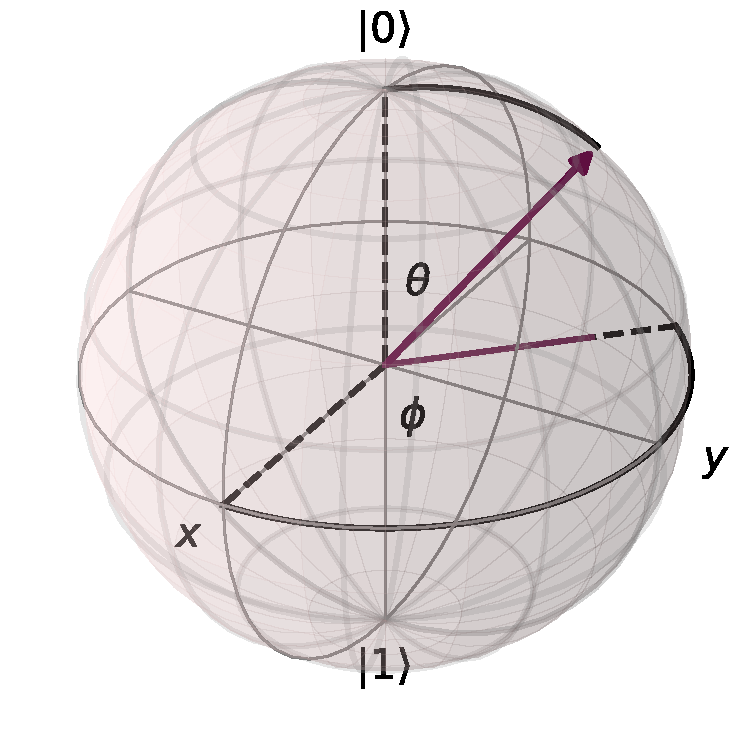
\includegraphics[]{Figs/Theory/bloch_sphere.pdf}
    \caption{Representation of a qubit state on the Bloch sphere. The angles $\phi$ and $\theta$ are displayed along with the projection onto the x-y plane.}
    \label{fig:bloch_sphere}
\end{marginfigure}

% \section{Time Evolution of a Quantum System}
% As a physics student, one is often met early in ones career by Newtons second law, stating that acceleration equals force times mass $\Vec{F} = m \Vec{a}$. Knowing the force asserted on an object thus gives the equations of motion. Often it is however more beneficial to represent the equations of motions in the Hamiltonian formalism, where one can derive the equations of motion by the energy of the system (the Hamiltonian). The equation of motions are now given by a coordinate and the canonical momentum to that coordinate. 

% In this formalism the time dependence of the coordinates $q$ and canonical momentum $p$ is given by\footnote{The canonical momentum is found from the Lagrangian which is related to the Hamiltonian by a Legendre transformation} :

% \begin{align}
%     \dot{p} = - \pfrac{}{q} &H(p, q) \\
%     \dot{q} = \pfrac{}{p} &H(p, q)
% \end{align}

% Or for a general function of a set of coordinates and the set of canonical momenta $f(\{q_i\}, \{p_i\}, t)$, we can represent the time-dependence using Poisson brackets: \cite{Fetter_continous_mechanics}
% \marginnote{A Poisson bracket refers to a specific combination of differentials. With $\{F, G\} = \sum_i \left(\pfrac{F}{q_i} \pfrac{G}{p_i} - \pfrac{F}{p_i} \pfrac{G}{q_i} \right)$} 

% \begin{equation}
%     \dot{f} = -\{H, f\} + \pfrac{}{t} f 
% \end{equation}

% \paragraph{Going Quantum - }
% From the Hamiltonian formalism the switch to quantum mechanics is significantly shorter. By first introducing the commutator between two operators: \todo{Introduce operators above with operators and uncertainty principle}
% \begin{equation}
%     \comm{A}{B} = AB - BA
% \end{equation}

% Now making the mapping from Poisson brackets to commutators with the appropiate prefactor, we find the correspondence principle:

% \begin{equation}
%     \{A, B\} \to \frac{\hbar}{i} \comm{A}{B}
% \end{equation}

% Such that the time dependence of an operator is given by:
% \begin{equation}
%     \dot{A} = \frac{i}{\hbar} \comm{H}{A} + \pfrac{}{t} A
% \end{equation}

% \textbf{Get to Schödingers Equation here}

% \textbf{Maybe introduce like this instead} \\ \noindent
\section{Time Evolution of a Quantum System}\label{sec:scroedinger}
Let us now take a look at how quantum systems change in time. A transformation from one state into another must leave the inner product unchanged to keep the normalization. This can be achieved by a unitary transformation\footnote{For unitary transformations we have: $\unitary^{-1} = \unitary^\dagger$ or equally $\unitary^\dagger\unitary = \identity$}. To see how a state at $t = t_0$ changes into a later time $t = t_0 + \Delta t$, we will have to find a unitary operator, $\mathcal{U}(\Delta t)$. To keep normalization, the transformation should satisfy:
\begin{equation}
    \braket{\psi; t_0}{\psi; t_0} = \braket{\psi; t_0 .. \Delta t}{\psi; t_0 .. \Delta t} = \mel{\psi; t_0}{\unitary^\dagger (\Delta t) \unitary(\Delta t)}{\psi; t_0} 
\end{equation}
which is satisfied since $\unitary$ is unitary. An additional requirement on the transformation is that the state should remain unchanged if no time has passed: $\unitary(\Delta t) \to \identity$ when $\Delta t \to 0$. By expanding the unitary operator around $\Delta t = 0$, and taking the limit $\Delta t \to dt$, these conditions are satisfied by:
\begin{equation}\label{eq:infinitesimal_time_evolution}
    \unitary(dt) = \identity - i \Omega dt
\end{equation}
Where $\Omega$ is a hermitian operator with units of frequency\footnote{To see why this keeps the normalization, we write $\unitary^\dagger(dt)\unitary(dt) = (\identity + i \Omega dt)(\identity - i \Omega dt) = \identity + dt^2 \Omega^2$ which goes to identity in the limit of $dt \to 0$ as the $dt^2$ term vanishes.}. 
Since the Hamiltonian generates time evolution in classical mechanics are it is not so strange that it does the in quantum mechanics. The actual operator : $\Omega = \frac{H}{\hbar}$. From eq. \ref{eq:infinitesimal_time_evolution} and by defining $\ket{\psi; t..dt} - \ket{\psi; t} = d\ket{\psi; t}$ we find the Schrödinger equation by:
\begin{align}
    \ket{\psi; t..dt} &= \unitary(dt) \ket{\psi; t} = \left(\identity - i \frac{H}{\hbar}   dt\right) \ket{\psi} \\
    \ket{\psi; t..dt} - \ket{\psi; t} &= i \frac{H}{\hbar}   dt \ket{\psi} \\
    i \hbar \frac{d}{dt}\ket{\psi} &=  H \ket{\psi}
\end{align}
Which is known as the Schrodinger's equation and governs unitary time evolution of quantum mechanical system given that it is closed from the environment and is not measured \cite{sakurai_modern_2021}. Two problems which we will return to in great detail.

If the Hamiltonian is independent of time, we can express the time evolution operator as:
\begin{equation}
    \unitary(\Delta t) = e^{-iH\Delta t/\hbar}
\end{equation}
which entirely removes the time-dependence from the state such that $\ket{\psi; t} = \unitary(t)\ket{\psi; t = 0}$.
If on the contrary, the Hamiltonian is dependent on time and commutes at different times, we can write it as:
\begin{equation}
    \unitary(\Delta t)\ket{\psi; t_0} = \exp\left(-\frac{i}{\hbar}\int_{t_0}^{t_0 + \Delta t} dt H(t)\right)\ket{\psi; t_0}
\end{equation}
If the Hamiltnoian at different times do not commute with itself, one could introduce the Dyson series\cite{sakurai_modern_2021}, another approach is to solve the differential equations numerically.

\subsection{Numerical Implementations}\label{sec:numerical_implementations}
The Schrodinger equation gives a simple linear relation between the time derivative, the state and the Hamiltonian. If we represent the states and the Hamiltonian as vectors and a matrix and naively let the infinitesimal time step go be of finite size: $dt\to\Delta t$, we could simply update the state by:
\begin{equation}
    \Vec{\psi}(t + \Delta t) =  \Vec{\psi}(t) - \frac{i\Delta t}{\hbar}\boldsymbol{H} \Vec{\psi}(t)
\end{equation}
Of course this is a crude approximation, which we could make better by splitting $\Delta t$ up into multiple pieces and applying the formula multiple times. While this method (Euler integration, see example in figure \ref{fig:euler_integration}) is simple to implement quickly loses precision if the time steps become large. Instead of solving this by increasing the amount of steps, we can instead look at more sophistaced algorithms.
\begin{marginfigure}
    \centering
    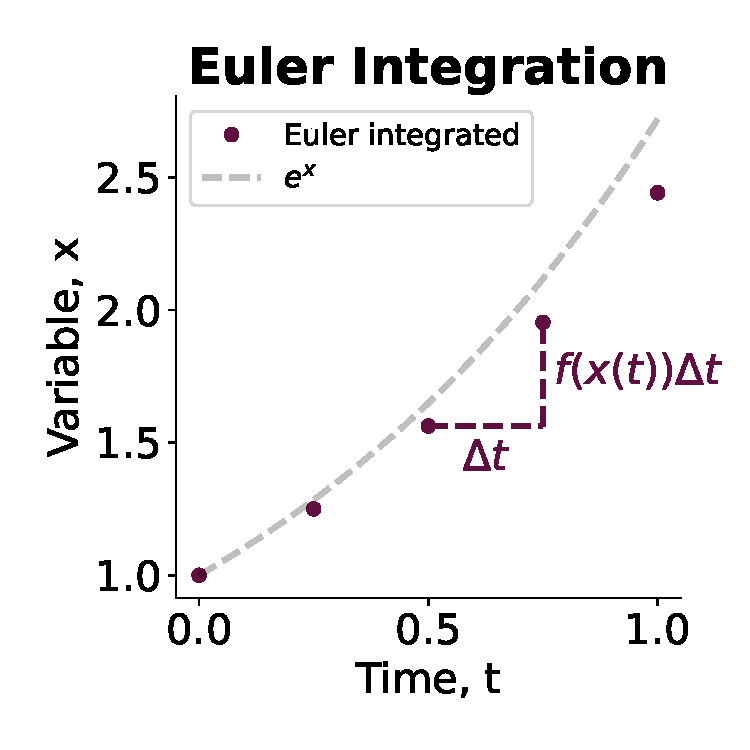
\includegraphics[]{Figs/Theory/euler_integration.pdf}
    \caption{Example of Euler integration $x'(t) = x$}
    \label{fig:euler_integration}
\end{marginfigure}


In the Qutip Library\cite{johansson_qutip_2012} , which we will use throughout this thesis, the Schroedinger equation is integrated by the Adams method. Here we will consider the last $n$ points in order to also approximate the higher order differentials of the function. If we have a differential equation:
\begin{equation}
    y'(t) = f(y(t))
\end{equation}
We can approximate the point $y(t+\Delta t)$ by a Taylor expanding around $t$:
\begin{equation}
    y(t) + \Delta t y'(t) + \frac12 \Delta t^2 y''(t) + \frac{1}{3!} \Delta t^3 y'''(t)\dots 
\end{equation}
The idea in the Adams algorithm is to approximate the differential up to order $n$ by using finite difference methods. The second order derivative can then be approximated by:
\begin{equation}
    y'(t) = f(t), \quad y''(t) = \frac{f(y(t)) - f(y(t - \Delta t))}{\Delta t} 
\end{equation}
And the third order differential by:
\begin{equation}
    y'''(t) = \frac{y''(t) - y''(t-\Delta t)}{\Delta t} = \frac{f(y(t)) - f(2y(t-\Delta t)) + f(y(t-2\Delta t))}{\Delta t^2}
\end{equation}


\begin{marginfigure}
    \centering
    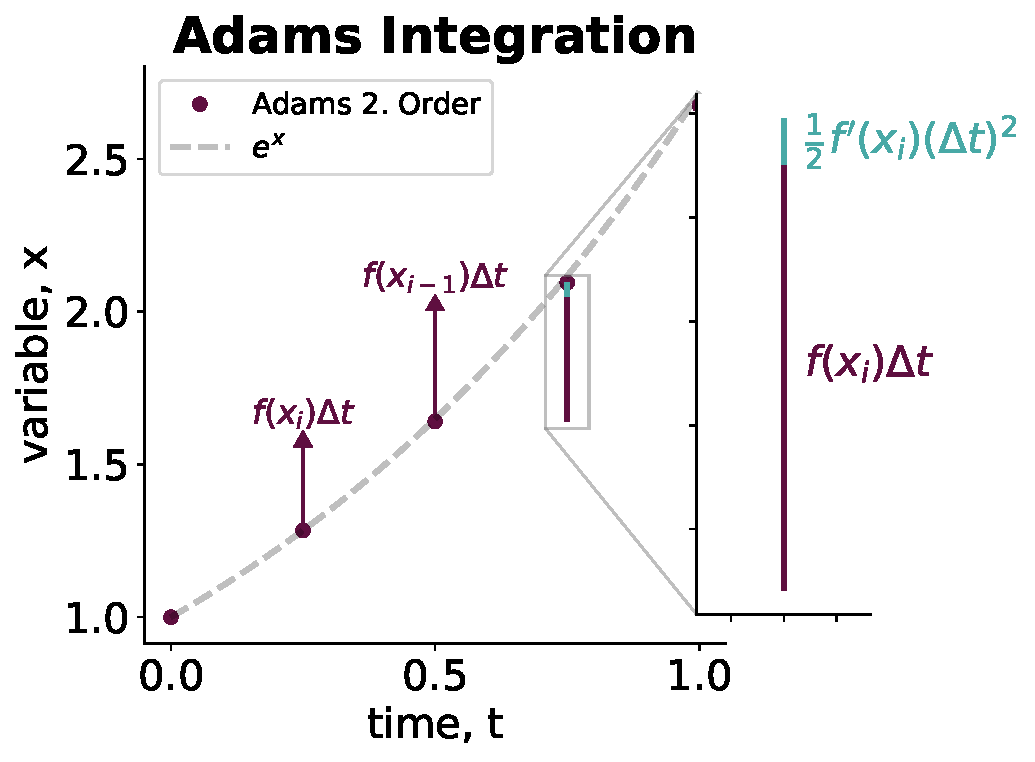
\includegraphics[width = 1.2 \linewidth]{Figs/Theory/adams_intergation.pdf}
    \caption{How the Adams algorithm works. Here the second order derivative is found by the finite difference method to be $f'(x_i) = (f(x_i) - f(x_{i-1}))/\Delta t$}
    \label{fig:Adams integration}
\end{marginfigure}
\todo{The label need to be switched!}
and onwards. A visualization of the second order method can be seen in figure \ref{fig:Adams integration}. The computation of the Adams algorithm is more precise since it considers higher order terms and it runs fast since it reuses the old calculations. Thus we just have to do one operation\footnote{in the sense that no operation has to wait for another operation before it can be run.} for calculating the next value of $y$. One challenge is that the algorithm requires $n$ points to get started. Thus we can either assume that every differential beyond order $m$ is $0$ when calculating the $0$th point. Such that we effectively would do an Euler integration for the first point, a second order Adams for the second and so on. The default order of the methods in this thesis will be order 12, so this way we lose a lot of precision in the beginning. Alternatively, we can use another algorithm which moves forward in time to approximate the higher order differentials. An example of such an algorithms is the Runge-Kutta method.

\todo{Check with source here: \url{https://link.springer.com/book/10.1007/978-3-540-78862-1} should be accessible within KU }
% \textit{The Runge-Kutta method goes forward in time to find intermediate time steps, where the differential equation again is evaluated. When summing the different paths, the errors cancel out up the order $n$, where $n$ is the amount of intermediate steps. To second order, the Runge-Kutta algorithm calculates half a time step: $k_1 = \Delta t / 2 \psi$ and averages the slope of the slope of the given point and the next. 
% }
% $ takes $\Vec{\psi_i} = \Vec{\psi_{i-1}} + k_1 + \mathcal{O}(\Delta t^3)$. To higher orders this lets us suppress the error for the first few steps using multiple steps with the Runge-Kutte method and when we have the first $n$ values, we can switch to the Adams method to improve speed while keeping the error small. \todo{Same source as above? } 
% \todo{Write this properly}
% \paragraph{Adams method} includes the values calculated in the last few steps to determine a polynomial expansion. This does not require to calculate as many points as the Runge-Kutta and comes with a high precision as well. Requires a few points to start, but one could use Runge-Kutta to find the first few points or run the algorithm backwards in time. 


% The Adam package is also the one used in the Qutip package which is used for this thesis. Here the algorithm is run to 12 order with a set error tolerance and the possibility to adapt and take multiple steps between the desired resolution.

\section{Computational Framework of the Thesis}
\begin{figure}[b]
    \centering
    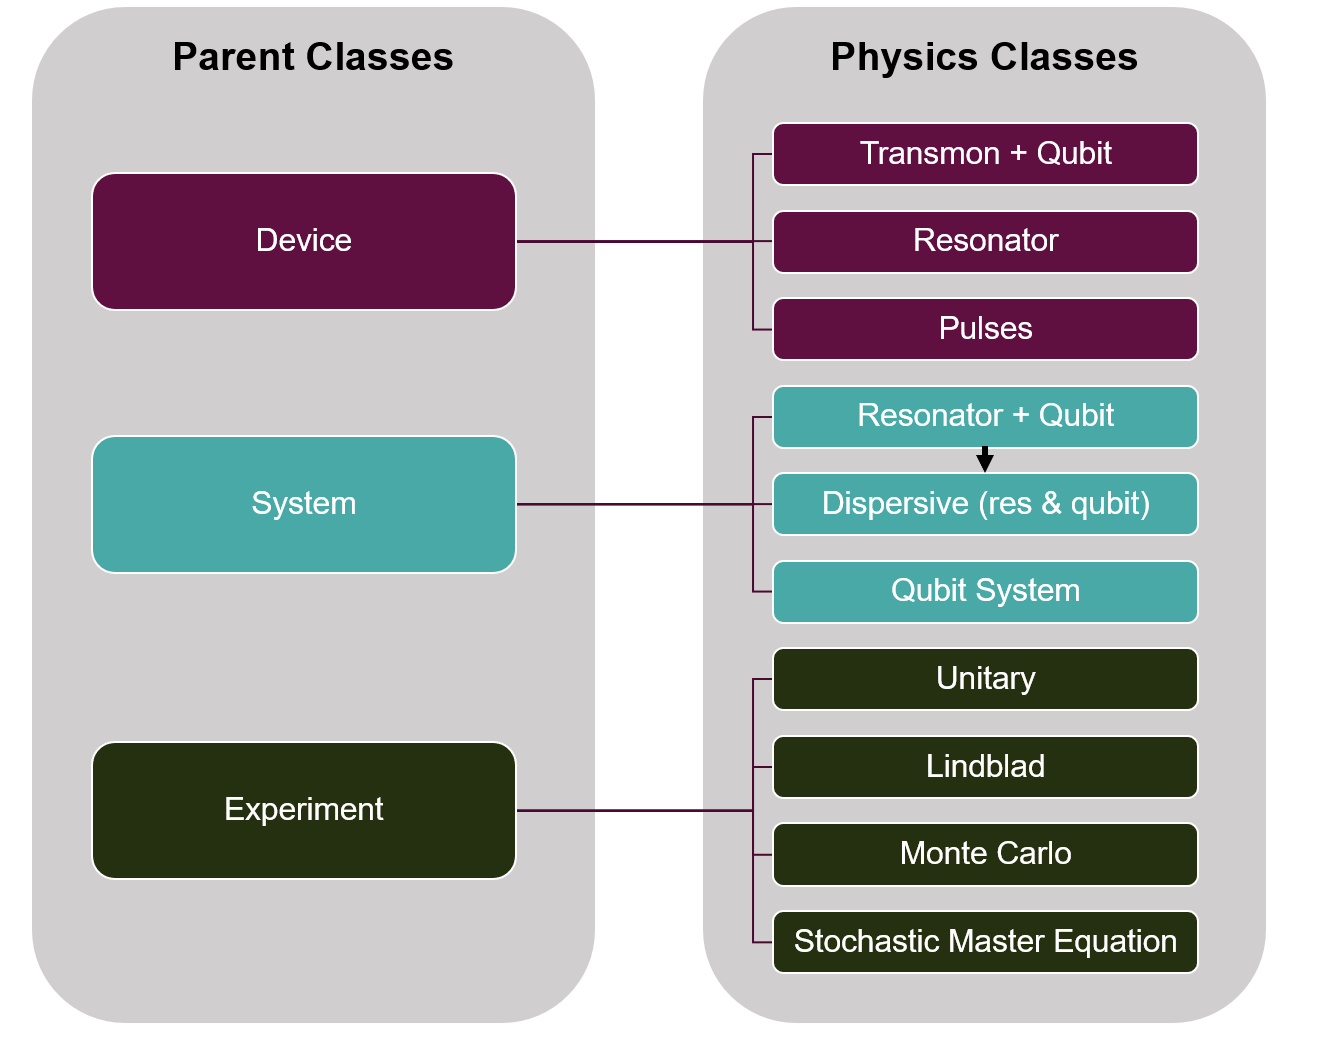
\includegraphics[width = 0.9 \textwidth]{Figs/Sections/Introduction/module_v2.png}
    \caption{Module structure divided into the Parent Classes maintainining parameters and sweeping and the Phyics classes which serves as containers for Hamiltonian, dissipation operators or simulation schemes.}
    \label{fig:module_overview}
\end{figure}
It is by no means a new idea to solve quantum mechanical problems by numerical simulations, so multiple well-optimized and versatile libraries exist. In this thesis, we base most of our calculations on the integration method present in the Qutip Library \cite{johansson_qutip_2012}. To make faster progress and hopefully contribute to the software in the laboratory, a module to make numerical superconducting qubit experiments was developed during this project. The package is a wrapper around the Qutip Library, but eases the setup of of calculating Hamiltonians of superconducting systems, running simulations and managing data. The documentation for the module QuantumDeviceSimulation can be found in appendix \ref{chap:code_documentation}.

An overview of the module is shown in figure \ref{fig:module_overview}. In general, it is built in three main parts:
\begin{itemize}
    \item \textbf{Devices} are the physical devices placed in the system. This includes different qubits, resonators and pulses.
    \item \textbf{Systems} are combinations of devices along with descriptions of how they interact.
    \item \textbf{Experiments} are organizing the different sweeps of parameters and applying the proper integration technique. 
\end{itemize}